\section{Preliminaries}
\label{sec::preliminaries}

We work with grids consisting of W$\times$H square cells.  Each cell is an
open set of points that are either all \emph{traversable} or all
\emph{non-traversable}.  Edges in the grid are horizontal or veritcal
transitions between the corners of square cells. We model edges as open
intervals of \emph{intermediate points}.  There are several other types of
points which are interesting. These are shown in Figure~\ref{fig::points}.
%\begin{figure}[h]
%\center
%		   \includegraphics[width=0.55\columnwidth]
%			{images/types_of_points.pdf}
%	\vspace{-3pt}
%       \label{fig::points}
%       \caption{Types of Points.}
%\end{figure}

%\end{minipage}
%

In this work we want to compute paths which are sequences of points of the
type $\langle p_1, \ldots\, p_k\rangle$. In particular we want each path to
have the property that every point $p_i$ is \emph{visible} from both $p_{i-1}$
and $p_{i+1}$.  Examples involving pairs of points that are both visible and
non-visible  are shown in Figure~\ref{fig::visibility}.
For further details refer to~\cite{haraborG13}.

\begin{figure}[hb]
\begin{minipage}[tb]{0.95\columnwidth}
\center
		   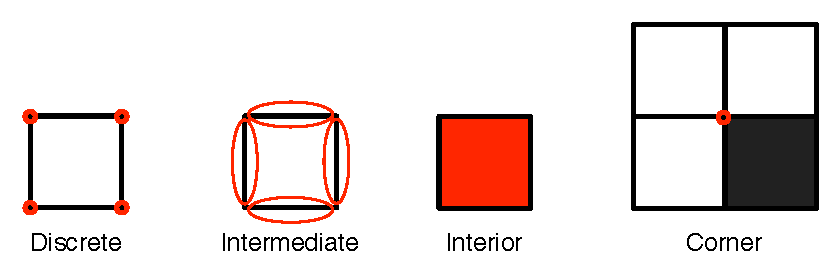
\includegraphics[width=0.45\columnwidth]
			{images/types_of_points.pdf}
	\vspace{-3pt}
       \label{fig::points}
       \caption{Types of Points.}
\end{minipage}
\begin{minipage}[tb]{0.95\columnwidth}
\center
		   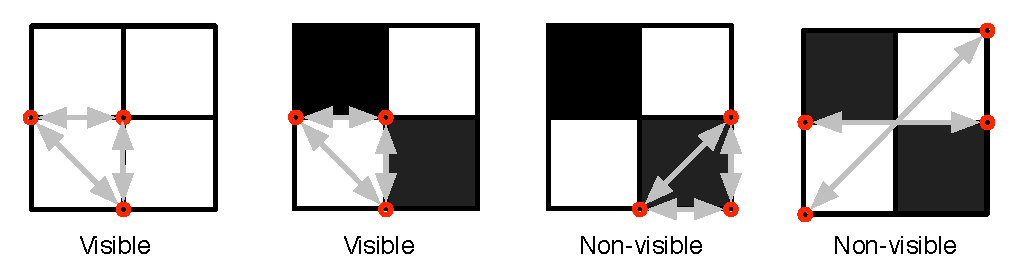
\includegraphics[width=0.55\columnwidth]
			{images/visibility.pdf}
	\vspace{-3pt}
       \label{fig::visibility}
       \caption{Examples of visible and non-visible pairs of points.}
\end{minipage}
\end{figure}
